\documentclass[aspectratio=169
  , xcolor={svgnames}
  , hyperref={ colorlinks,citecolor=Blue
             , linkcolor=DarkRed,urlcolor=DarkBlue}
  , usenames, dvipsnames
  , russian
  ]{beamer}


\usepackage{pgfpages}
\usepackage{graphicx}   % for 
\includegraphics{file.pdf}

\makeatletter
\@ifclassloaded{beamer}{
  % get rid of header navigation bar
  \setbeamertemplate{headline}{}
  % get rid of bottom navigation symbols
  \setbeamertemplate{navigation symbols}{}
  % get rid of footer
  %\setbeamertemplate{footline}{}
}
{}
\makeatother
%%%%%%%%%%%%%%%%%%%%%%%%%%%%%%%%%%%%%%%%%%%%%
\usepackage{fontawesome}
% \newfontfamily{\FA}{Font Awesome 5 Free} % some glyphs missing
\expandafter\def\csname faicon@facebook\endcsname{{\FA\symbol{"F09A}}}
\def\faQuestionSign{{\FA\symbol{"F059}}}
\def\faQuestion{{\FA\symbol{"F128}}}
\def\faExclamation{{\FA\symbol{"F12A}}}
\def\faUploadAlt{{\FA\symbol{"F093}}}
\def\faLemon{{\FA\symbol{"F094}}}
\def\faPhone{{\FA\symbol{"F095}}}
\def\faCheckEmpty{{\FA\symbol{"F096}}}
\def\faBookmarkEmpty{{\FA\symbol{"F097}}}

\newcommand{\faGood}{\textcolor{ForestGreen}{\faThumbsUp}}
\newcommand{\faBad}{\textcolor{red}{\faThumbsODown}}
\newcommand{\faWrong}{\textcolor{red}{\faTimes}}
\newcommand{\faMaybe}{\textcolor{blue}{\faQuestion}}
\newcommand{\faCheckGreen}{\textcolor{ForestGreen}{\faCheck}}
%%%%%%%%%%%%%%%%%%%%%%%%%%%%%%%%%%%%%%%%%%%%%

\usepackage{fontspec}
\usepackage{xunicode}
\usepackage{xltxtra}
\usepackage{xecyr}
\usepackage{hyperref}

\setmainfont[
 Ligatures=TeX,
 Extension=.otf,
 BoldFont=cmunbx,
 ItalicFont=cmunti,
 BoldItalicFont=cmunbi,
% Scale = 1.1
]{cmunrm}
\setsansfont[
 Ligatures=TeX,
 Extension=.otf,
 BoldFont=cmunsx,
 ItalicFont=cmunsi,
%  Scale = 1.2
]{cmunss}
%\setmainfont[Mapping=tex-text]{DejaVu Serif}
%\setsansfont[Mapping=tex-text]{DejaVu Sans}
%\setmonofont{Fira Code}[Contextuals=AlternateOff]
\setmonofont{Fira Code}[Contextuals=Alternate,Scale=0.9]
\newfontfamily{\myfiracode}[Scale=1.5,Contextuals=Alternate]{Fira Code}
%\setmonofont[Scale=0.9,BoldFont={Inconsolata Bold}]{Inconsolata}

\usepackage{polyglossia}
\setmainlanguage{russian}
\setotherlanguage{english}


%\newfontfamily\dejaVuSansMono{DejaVu Sans Mono}
% https://github.com/vjpr/monaco-bold/raw/master/MonacoB/MonacoB.otf
%\newfontfamily\monacoB{MonacoB}
%%%%%%%%%%%%%%%%%%%%%%%%%%%%%%%%%%%%%%%%%%%%%%%5
\usepackage{soul} % for \st that strikes through
\usepackage[normalem]{ulem} % \sout

\usepackage{stmaryrd}
\newcommand{\sem}[1]{\ensuremath{\llbracket #1\rrbracket}}


\usepackage{listings}
%\lstdefinestyle{style1}{
%  language=haskell,
%  numbers=left,
%  stepnumber=1,
%  numbersep=10pt,
%  tabsize=4,
%  showspaces=false,
%  showstringspaces=false
%}
%\lstdefinestyle{hsstyle1}
%{ language=haskell
%%          , basicstyle=\monacoB
%         , deletekeywords={Int,Float,String,List,Void}
%         , breaklines=true
%         , columns=fullflexible
%         , commentstyle=\color{ForestGreen}
%         , escapeinside=§§
%         , escapebegin=\begin{russian}\commentfont
%         , escapeend=\end{russian}
%         , commentstyle=\color{ForestGreen}
%         , escapeinside=§§
%         , escapebegin=\begin{russian}\color{ForestGreen}
%         , escapeend=\end{russian}
%         , mathescape=true
%%          , backgroundcolor = \color{MyBackground}
%}
%
%\newcommand{\inline}[1]{\lstinline{haskell}{#1}}
%\def\hsinline{\mintinline{haskell}}
%\def\inline{\hsinline}
%
%\lstnewenvironment{hslisting} {
%    \lstset { style={hsstyle1} }
%  }
%  {}
%  
%%%%%%%%%%%%%%%%%%%%%%%%%%%%%%%%%%%%%%%%%%%%%%%%%%%%%%%%%%%  
%%\setmainfont[
%% Ligatures=TeX,
%% Extension=.otf,
%% BoldFont=cmunbx,
%% ItalicFont=cmunti,
%% BoldItalicFont=cmunbi,
%%]{cmunrm}
%%% С засечками (для заголовков)
%%\setsansfont[
%% Ligatures=TeX,
%% Extension=.otf,
%% BoldFont=cmunsx,
%% ItalicFont=cmunsi,
%%]{cmunss}
%% \setmonofont[Scale=0.6]{Monaco}
%
%\usefonttheme{professionalfonts}
%\usepackage{times}
\usepackage{tikz}
\usetikzlibrary{cd}
\usepackage{tikz-cd}
\usepackage{caption}
\usepackage{subcaption}

%\renewtheorem{definition}{برهان}[chapter]
%%\DeclareMathOperator{->}{\rightarrow}
%\newcommand\iso{\ensuremath{\cong}}
%\usepackage{verbatim}
%\usepackage{graphicx}
%\usetikzlibrary{arrows,shapes}

%\usepackage{amsmath}
%\usepackage{amsfonts}
\usepackage{scalerel}
\DeclareMathOperator*{\myvee}{\scalerel*{\vee}{\sum}}
\DeclareMathOperator*{\mywedge}{\scalerel*{\wedge}{\sum}}

%
%\usepackage{tabulary}
%
%% sudo aptget install ttf-mscorefonts-installer
%%\setmainfont{Times New Roman}
%%\setsansfont[Mapping=tex-text]{DejaVu Sans}
%
%%\setmonofont[Scale=1.0,
%%    BoldFont=lmmonolt10-bold.otf,
%%    ItalicFont=lmmono10-italic.otf,
%%    BoldItalicFont=lmmonoproplt10-boldoblique.otf
%%]{lmmono9-regular.otf}
%
\usepackage[cache=true]{minted}
\usemintedstyle{perldoc}

\def\hsinline{\mintinline{haskell}}
\def\mlinline{\mintinline{ocaml}}
% color options
\definecolor{YellowGreen} {HTML}{B5C28C}
\definecolor{ForestGreen} {HTML}{009B55}
\definecolor{MyBackground}{HTML}{F0EDAA}



\institute{матмех СПбГУ}

\addtobeamertemplate{title page}{}{
  \begin{center}{\tiny Дата сборки: \today}\end{center}
}





\newcommand{\head}[2]{\multicolumn{1}{>{\centering\arraybackslash}m{#1}}{\textbf{\small #2}}}


\title{Staged Selective парсер-комбинаторы}
\subtitle{Staged Selective Parser Combinators}

\date{1 марта 2021}
\author{Косарев Дмитрий} 
\institute[]{\normalfont
По статье <<Staged Selective Parser Combinators>> \\c конференции
IFCP 2020}


\AtBeginSection[]
{
  \begin{frame}<beamer>
    \frametitle{Оглавление}
    \tableofcontents[currentsection,currentsubsection]
  \end{frame}
} 
\AtBeginSubsection[]
{
  \begin{frame}<beamer>
    \frametitle{Оглавление}
    \tableofcontents[ currentsection
                    , currentsubsection
                    ]
  \end{frame}
}
\begin{document}

% Title page 
\begin{frame}
   \tikz [overlay] {
    \node at
        ([yshift=-10cm,xshift=-2cm]current page.east) 
        {
\includegraphics[height=2cm]{pictures/SPbGU_Logo.png}};
    \node at
        ([yshift=-10cm,xshift=2cm]current page.west) 
        {
\includegraphics[height=1.5cm]{pictures/jetbrainsResearch.pdf}};
   }
   \titlepage
\end{frame}



% For every picture that defines or uses external nodes, you'll have to
% apply the 'remember picture' style. To avoid some typing, we'll apply
% the style to all pictures.
%\tikzstyle{every picture}+=[remember picture] 

% By default all math in TikZ nodes are set in inline mode. Change this to
% displaystyle so that we don't get small fractions.
\everymath{\displaystyle}

\section{Парсер-комбинаторы (кратко)}


\defverbatim[colored]{\haskellPrimA}{
\begin{minted}{haskell}
item :: Parser Char 
item = satisfy (const True)
char :: Char -> Parser Char 
char c = satisfy (==c)
\end{minted}
}
\defverbatim[colored]{\haskellPrimB}{
\begin{minted}{haskell}
eof :: Parser ()
eof = notFollowedBy item
\end{minted}
}

\begin{frame}[fragile]{Парсер-комбинаторы. Примитивные операции}
\begin{minted}{haskell}
satisfy :: (Char -> Bool) -> Parser Char 
\end{minted}
\uncover<2->{
\haskellPrimA
}
\begin{minted}{haskell}
try :: Parser a -> Parser a 
lookAhead :: Parser a -> Parser a 
notFollowedBy :: Parser a -> Parser ()
\end{minted}
\uncover<2->{
\haskellPrimB
}
\end{frame}

\begin{frame}[fragile]
\begin{minipage}{0.65\linewidth}
\begin{minted}{haskell}
class Functor (f :: * -> *) where
  fmap :: (a -> b) -> f a -> f b

-- application abstracted 
class Functor f => Applicative f where
  -- | Lift a value.
  pure :: a -> f a
  -- | Sequential application.
  (<*>) :: f (a -> b) -> f a -> f b

-- Nondeterminism (or try-catch) abstracted
class Applicative f => Alternative f where
  -- | The identity of '<|>'
  empty :: f a
  -- | An associative binary operation
  (<|>) :: f a -> f a -> f a
\end{minted}
\end{minipage}\hspace{1cm}
\begin{minipage}{0.2\linewidth}
Монад пока нет, это нарочно
\end{minipage}
\end{frame}


\begin{frame}[fragile]
\begin{block}{\emph{Идея парсер-комбинаторов}}
Использовать обычные функции, чтобы строить большие парсеры
\end{block}
\vspace{1em}

%\uncover<2->{
\begin{minted}{haskell}
char :: Char -> Parser Char 
\end{minted}
%}
\newln
\begin{minted}{haskell}
sequence :: Applicative f => [f a] -> f [a]
sequence = foldr (<:>) (pure [])

traverse :: Applicative f => (a -> f b) -> [a] -> f [b]
traverse f = sequence . map f  
\end{minted}
\newln

%\uncover<2->{
\begin{minted}{haskell}
string :: String -> Parser String 
string = traverse char 
\end{minted}
%}
\newln
\begin{minted}{haskell}
string :: String -> Parser String 
oneOf = foldr (<|>) empty . map char 
\end{minted}
%TODO: ещё слайд про предыдущеге из доклада?
\end{frame}

%%%%%%%%%%%%%%%%%%%%%%%%%%%%%%%%%%%%%%%%%%%%%%%%%%%%%%%%%%%%%%%
\section{Заслуги работы (библиотеки Parsley)}


\begin{frame}{Parsec vs. Parsley} 
\def\sad{\textcolor{red}{\Huge\faSadTear}}
\def\yolo{\textcolor{ForestGreen}{\Huge\faGrinStars}}

\Large 
\begin{center}
\renewcommand{\arraystretch}{2}
\begin{tabular}{c|cp{2cm}cccc}
 & Performance & Error messages & Grammar & Debugging & Analysis  \\
\hline
Parsec & \Huge \faMeh & \head{2cm}{\Huge \faMeh} & \yolo & \sad & \sad \\
\pause
Parsley &\Huge  \faGood & \head{2cm}{\Huge 404} & \yolo & \yolo & \Huge  \faGood \\
\end{tabular}
\renewcommand{\arraystretch}{1}
\end{center}
\pause
\newln 
Как этого удалось добиться? \emph{Метапрограммирование!} (Typed Template \Haskell{})
\end{frame}

%\begin{frame}[fragile]{11}
%\includegraphics[page=0]{pipeline}
%
%TODO: слайд с примером
%\end{frame}


\section{Monads  и Selectives}
\setminted{fontsize=\Large,baselinestretch=1}

\begin{frame}[fragile]{Monad}
\begin{minted}{haskell}
class Applicative m => Monad (m :: * -> *) where
  -- | Inject a value into the monadic type.
  return      :: a -> m a
  return      = pure
  
  -- | Sequentially compose two actions, 
  -- passing any value produced
  -- by the first as an argument to the second.
  (>>=)       :: forall a b. m a -> (a -> m b) -> m b
\end{minted}
\end{frame}


\begin{frame}[fragile]
\begin{minted}{haskell}
satisfy :: (Char -> Bool) -> Parser Char 
satisfy p = item >>= (\c -> 
                        if p c then pure c 
                        else        empty)
  
ident :: Parser String 
ident = (satisfy isAlpha <:> 
         many (satisfy isAlphaNum) ) >>= (\c -> 
              if isKeyword c then empty
              else                pure c)
\end{minted}
\end{frame}

\begin{frame}[fragile]
\begin{minted}{haskell}
(>?>) :: Monad m => m a -> (a -> Bool) -> m a
m >?> f = m >>= \x -> if f x then pure x else empty
\end{minted}
\newln

\begin{minted}{haskell}
satisfy :: (Char -> Bool) -> Parser Char 
satisfy p = item >?> p
  
ident :: Parser String 
ident = (satisfy isAlpha <:> 
         many (satisfy isAlphaNum) ) 
        >?> (not . isKeyword)
\end{minted}
\end{frame}

\setminted{fontsize=\normalsize,baselinestretch=1}


\begin{frame}
\begin{center}
\Large
Монады классные, что же с ними не так и зачем нужны Selective функторы?
\end{center}
\end{frame}

\setminted{fontsize=\Large,baselinestretch=1}
\begin{frame}[fragile]{Selective}
\begin{minted}{haskell}
-- case expression abstracted
class Applicative f => Selective f where
  -- In the original paper 
  select :: f (Either a b) -> f (a -> b) -> f b
  
  -- alternative definition, used by Parsley
  branch :: f (Either a b) -> f (a -> c) -> f (b -> c) 
         -> f c
\end{minted}
\end{frame}



\begin{frame}[fragile]{Реализация \mintinline{haskell}{>?>}}
\Large
С помощью \mintinline{haskell}{Monad}
\begin{lstlisting}[language=haskell
  , basicstyle=\Large\ttfamily
  , escapeinside={!}{!}
  ]
(>?>) :: Monad m => m a -> (a -> Bool) -> m a
m >?> f = m >>= !\tikzmark{a}! \ x -> if f x then pure x else empty !\tikzmark{b}!
\end{lstlisting}
\begin{tikzpicture}[remember picture,overlay]
  \draw[red,rounded corners]
    ([shift={(-3pt,2ex)}]pic cs:a) 
      rectangle 
    ([shift={(3pt,-0.65ex)}]pic cs:b);
\end{tikzpicture}
\pause 

С помощью \mintinline{haskell}{Selective}
\begin{lstlisting}[language=haskell
  , basicstyle=\Large\ttfamily
  , escapechar=!
  , mathescape=false
  ]
(>?>) :: Selective m => m a -> (a -> Bool) -> m a
m >?> f = select ( !\tikzmark{c}!(\ x -> !\tikzmark{d}!
!\tikzmark{e}!  if f x then Right () 
  else        Left ()) !\tikzmark{f}!   <$> fx) empty 
\end{lstlisting}
\begin{tikzpicture}[remember picture,overlay]
\draw[red,rounded corners]
  ([shift={(-3pt,2.5ex)}]pic cs:c) 
    rectangle 
  ([shift={(3pt,-0.5ex)}]pic cs:d);
\draw[red,rounded corners]
  ([shift={(-3pt,2.2ex)}]pic cs:e) 
    rectangle 
  ([shift={(3pt,-0.65ex)}]pic cs:f);
\end{tikzpicture}
% Со второй реализацией статически знаем больше 
\end{frame}

\begin{frame}[fragile]{Чего не умеют \mintinline{haskell}{Selective}?}
\Large 
\begin{itemize}
\item Использовать несколько предыдущих результатов

  \lstinline[language=haskell, basicstyle=\Large\ttfamily]{mf >>= \ f -> mg >>= \ g -> mh >>= \ h -> ... }
\item Монадический join:

 \lstinline[language=haskell, basicstyle=\Large\ttfamily]{join :: m (m a) -> m a}
\end{itemize}
\newln 

\begin{block}{Замечание}
Если \mintinline{haskell}{Selective} не умеют \mintinline{haskell}{join}
или \mintinline{haskell}{Applicative} не умеют КЗ-грамматики, то это не значит, что работающий парсер нельзя написать.
\end{block}
\end{frame}


\setminted{fontsize=\normalsize,baselinestretch=1}



\section{Превращение монадического парсера в аппликативный}
\subsection{chainr1}

\setminted{fontsize=\Large,baselinestretch=1}
\defverbatim[colored]{\haskellChainrA}{
\begin{minted}{haskell}
chainr1 :: Parser a -> Parser (a -> a -> a) -> Parser a
chainr1 p op = scan
  where
    scan     = do { x <- p; rest x }
    rest x   = do { f <- op
                  ; y <- scan
                  ; return (f x y)
                  }
              <|> return x
\end{minted}
}


\defverbatim[colored]{\haskellChainrB}{
\begin{minted}{haskell}
chainr1 p op = p >>= rest
  where
  
    rest x = (op >>= \f ->
              chainr1 p op >>= \y ->
              pure (f x y))
            <|> pure x
\end{minted}
}

\defverbatim[colored]{\haskellChainrC}{
\begin{minted}[escapeinside=!!]{haskell}
chainr1 :: Parser a -> Parser (a -> a -> a) -> Parser a
chainr1 p op = p <**> rest
  where
    rest :: Parser (a -> a)
    -- N.B. arguments must go away   
    rest !\textcolor{red}{x}! = (op >>= \f ->
              chainr1 p op >>= \y ->
              pure (!\textcolor{red}{f x y}!))
            <|> pure x
          
-- (<**>) :: Applicative f => f a -> f (a -> b) -> f b
\end{minted}
}

\defverbatim[colored]{\haskellChainrD}{
\begin{minted}{haskell}
chainr1 :: Parser a -> Parser (a -> a -> a) -> Parser a
chainr1 p op = p <**> rest
  where

    rest   = (op >>= \f ->
              chainr1 p op >>= \y ->
              pure (flip f y))
            <|> pure id
          
-- Уже компилируется, но надо избавиться от двух >>=
-- и это очень просто
\end{minted}
}

\defverbatim[colored]{\haskellChainrE}{
\begin{minted}{haskell}
chainr1 :: Parser a -> Parser (a -> a -> a) -> Parser a
chainr1 p op = p <**> rest
  where

    rest   = (flip <$> op <*> chainr1 p op)
            <|> pure id
            
-- C chainr1 всё

-- С chainl1 будет посложнее            
\end{minted}
}

%%% Now chainl 


\defverbatim[colored]{\haskellChainlA}{
\begin{minted}{haskell}
chainl1 :: Parser a -> Parser (a -> a -> a) -> Parser a
chainl1 p op = do { x <- p; rest x }
  where
    rest x   = do { f <- op
                  ; y <- p
                  ; rest (f x y)
                  }
                <|> return x
\end{minted}
}

\defverbatim[colored]{\haskellChainlB}{
\begin{minted}{haskell}
chainl1 :: Parser a -> Parser (a -> a -> a) -> Parser a
chainl1 p op = p >>= rest
  where
  
    rest x  = op >>= \f ->
              p  >>= \y ->
              rest (f x y)
              <|> return x
\end{minted}
}

\defverbatim[colored]{\haskellChainlC}{
\begin{minted}[escapeinside=!!]{haskell}
chainl1 :: Parser a -> Parser (a -> a -> a) -> Parser a
chainl1 p op = p !\textcolor{ForestGreen}{<**>}! rest
  where
    -- N.B. Аргумент нужно убирать
    rest !\textcolor{red}{x}!  = op >>= \f ->
              p  >>= \y ->
              rest (!\textcolor{red}{f x y}!)
              <|> return !\textcolor{ForestGreen}{id}!
              
-- рекурсивный вызов мешает
-- Интуиция: реализуем foldl через foldr
\end{minted}
}
\defverbatim[colored]{\haskellChainlD}{
\begin{minted}{haskell}
chainl1 :: Parser a -> Parser (a -> a -> a) -> Parser a
chainl1 p op = p <**> rest
  where
    
    rest   = (op >>= \f ->
              p  >>= \y ->
              (\ g x -> g (f x y)) <$> rest)
              <|> pure id
          
-- Теперь превратим (\ g x -> g (f x y)) в парсер, 
-- чтобы вытолкнуть rest наружу
\end{minted}
}

\defverbatim[colored]{\haskellChainlE}{
\begin{minted}{haskell}
chainl1 :: Parser a -> Parser (a -> a -> a) -> Parser a
chainl1 p op = p <**> rest
  where

    rest   = (op >>= \f ->
              p  >>= \y ->
              pure (\ g x -> g (f x y)) ) <*> rest
            <|> pure id
          
-- (<*>) :: Applicative f => f (a -> b) -> f a -> f b
\end{minted}
}


\defverbatim[colored]{\haskellChainlF}{
\begin{minted}{haskell}
chainl1 :: Parser a -> Parser (a -> a -> a) -> Parser a
chainl1 p op = p <**> rest
  where

    rest   = (op >>= \f ->
              p  >>= \y ->
              -- pure (\ g x -> g (f x y)) 
              -- pure (\ g x -> g (flip f y x)) 
              -- pure (\ g -> g . flip f y)) 
              pure (flip (.) (flip f y))
              ) <*> rest
            <|> pure id
\end{minted}
}

\defverbatim[colored]{\haskellChainlG}{
\begin{minted}{haskell}
chainl1 :: Parser a -> Parser (a -> a -> a) -> Parser a
chainl1 p op = p <**> rest
  where

    rest   = (op >>= \f ->
              p  >>= \y ->
              flip (.) <$> pure (flip f y))
              ) <*> rest
            <|> pure id
          
\end{minted}
}

\defverbatim[colored]{\haskellChainlH}{
\begin{minted}{haskell}
chainl1 :: Parser a -> Parser (a -> a -> a) -> Parser a
chainl1 p op = p <**> rest
  where

    rest   =  flip (.) <$> 
               (op >>= \f ->
                p  >>= \y ->
                pure (flip f y))
                ) <*> rest
            <|> pure id
          

\end{minted}
}

\defverbatim[colored]{\haskellChainlI}{
\begin{minted}{haskell}
chainl1 :: Parser a -> Parser (a -> a -> a) -> Parser a
chainl1 p op = p <**> rest
  where
    rest :: Parser (a -> a)
    rest =  
      flip (.) <$> (flip <$> op <*> chainl1 p op) <*> rest
      <|> pure id
          
-- Конец
\end{minted}
}

\setminted{fontsize=\normalsize,baselinestretch=1}


\begin{frame}[t]
\haskellChainrA
\end{frame}
\begin{frame}[t]
\haskellChainrB
\end{frame}
\begin{frame}[t]
\haskellChainrC
\end{frame}
\begin{frame}[t]
\haskellChainrD
\end{frame}
\begin{frame}[t]
\haskellChainrE
\end{frame}


\subsection{chainl1}

\begin{frame}[t]%{\haskellChainl}
\haskellChainlA
\end{frame}
\begin{frame}[t]
\haskellChainlB
\end{frame}
\begin{frame}[t]
\haskellChainlC
\end{frame}
\begin{frame}[t]
\haskellChainlD
\end{frame}
\begin{frame}[t]
\haskellChainlE
\end{frame}

\begin{frame}[t]
\haskellChainlF
\end{frame}
\begin{frame}[t]
\haskellChainlG
\end{frame}
\begin{frame}[t]
\haskellChainlH
\end{frame}
\begin{frame}[t]
\haskellChainlI
\end{frame}

%% %%%%%%%%%%%%%%%%%%%%%%%%%%%%%%%%%%%%%%%%%%%%%%%%%%%%%%%%%%%

\section{Законы}


\defverbatim[colored]{\lawApp}{
\begin{minted}{haskell}
    pure id <*> p = p                          -- (1)
pure f <*> pure x = pure (f x)                 -- (2)
     u <*> pure x = pure (λf -> f x) <*> u     -- (3)
  u <*> (v <*> w) = pure (.) <*> u <*> v <*> w -- (4)
\end{minted}
}

\defverbatim[colored]{\lawAlt}{
\begin{minted}{haskell}
(p <|> q) <|> r = p <|> (q <|> r) -- (5)
    empty <|> p = p <|> empty = p -- (6)
    empty <*> p = empty           -- (7)
   pure x <|> p = pure x          -- (8)
\end{minted}
}

\defverbatim[colored]{\lawSelParser}{
\begin{minted}{haskell}
branch (pure (Left  x)) p q = p <*> pure x                     -- (9)
branch (pure (Right y)) p q = q <*> pure y                     -- (10)
branch b (pure f) (pure g)  = pure (either f g) <*> b          -- (11)
        branch (x *> y) p q = x *> branch y p q                -- (12)
           branch b p empty = branch (pure swap <*> b) empty p -- (13)

branch (branch b empty (pure f)) empty k = branch (pure g <*> b) empty k 
  where
    g = either (const (Left ())) (either (const (Left ())) Right. f) -- (14)
\end{minted}
}

\begin{frame}[fragile]{Законы Applicative}
\setminted{fontsize=\large,baselinestretch=1}
\begin{minted}{haskell}
-- application abstracted 
class Functor f => Applicative f where
    -- | Lift a value.
    pure :: a -> f a
    -- | Sequential application.
    (<*>) :: f (a -> b) -> f a -> f b



    pure id <*> p = p                          -- (1)
pure f <*> pure x = pure (f x)                 -- (2)
     u <*> pure x = pure (λf -> f x) <*> u     -- (3)
  u <*> (v <*> w) = pure (.) <*> u <*> v <*> w -- (4)
\end{minted}
\end{frame}



\begin{frame}[fragile]{Законы Selective}
\setminted{fontsize=\large,baselinestretch=1}
\begin{minted}{haskell}
-- case expression abstracted
class Applicative f => Selective f where
  branch :: f (Either a b) -> f (a -> c) -> f (b -> c) -> f c
\end{minted}
%\begin{lstlisting}[language=haskell]
\newln 

\begin{minted}{haskell}
branch (pure (Left  x)) p q = p <*> pure x                     -- (9)
branch (pure (Right y)) p q = q <*> pure y                     -- (10)
branch b (pure f) (pure g)  = pure (either f g) <*> b          -- (11)
        branch (x *> y) p q = x *> branch y p q                -- (12)
           branch b p empty = branch (pure swap <*> b) empty p -- (13)
           
branch (branch b empty (pure f)) empty k = 
      branch (pure g <*> b) empty k  -- (14)
  where
    g = either (const (Left ())) (either (const (Left ())) Right. f) 
\end{minted}
%\end{lstlisting}

\end{frame}


\begin{frame}[fragile]{Законы Alternative}
\setminted{fontsize=\large,baselinestretch=1}
\begin{minted}{haskell}
-- Nondeterminism (or try-catch) abstracted
class Applicative f => Alternative f where
  -- | The identity of '<|>'
  empty :: f a
  -- | An associative binary operation
  (<|>) :: f a -> f a -> f a



(p <|> q) <|> r = p <|> (q <|> r) -- (5)
    empty <|> p = p <|> empty = p -- (6)
    empty <*> p = empty           -- (7)
   pure x <|> p = pure x          -- (8)
\end{minted}
\end{frame}



\begin{frame}[fragile]{Законы парсеров}
\setminted{fontsize=\large,baselinestretch=1}
\begin{minted}{haskell}
try (satisfy f) = satisfy f -- (15)
try (negLook p) = negLook p -- (16)

look empty       = empty    -- (17)
look (pure x)    = pure x   -- (18)
negLook empty    = pure ()  -- (19)
negLook (pure x) = empty    -- (20)

look (look p)       = look p                       -- (21)
look p <|> look q   = look (try p <|> q)           -- (22)
negLook (negLook p) = look p                       -- (23)
look (negLook p)    = negLook (look p) = negLook p -- (24)
-- de Morgan law where *> is conjunction
negLook (try p <|> q)   = negLook p *> negLook q     -- (25)
negLook p <|> negLook q = negLook (look p *> look q) -- (26)
\end{minted}
\end{frame}

\section{Реализация}
\setminted{fontsize=\normalsize,baselinestretch=1}

\begin{frame}[fragile,plain]{}
\includegraphics[page=2]{pipeline}
\begin{minted}{haskell}
newtype Fix (syn :: (* -> *) -> (* -> *)) (a :: *) where 
  In :: syn (Fix syn) a -> Fix syn a

newtype Parser a = Parser (Fix ParserF a)
data ParserF (k :: * -> *) (a :: *) where
  Pure :: a -> ParserF k a
  Satisfy :: (Char -> Bool) -> ParserF k Char
  Try :: k a -> ParserF k a
  Look :: k a -> ParserF k a
  NegLook :: k () -> ParserF k ()
  Empty :: ParserF k a
  Branch :: k (Either x y) -> k (x -> a) -> k (y -> a) -> ParserF k a
  (:<*>:) :: k (a -> b) -> k a -> ParserF k b
  (:*>:) :: k a -> k b -> ParserF k b
  (:<*:) :: k a -> k b -> ParserF k a
  (:<|>:) :: k a -> k a -> ParserF k a
\end{minted}
\end{frame}




\begin{frame}[fragile]{High level optimizer. Пример 1}
%\includegraphics[page=3]{pipeline}

\begin{minted}{haskell}
string :: String -> Parser String
string = traverse char
\end{minted}

\begin{minted}{haskell}
string "ab"
-- urolling
pure (:) <*> char 'a' <*> (pure (:) <*> char 'b' <*> pure [])
-- Applicative fusion optimizations ....
satisfy (== 'a') *> satisfy (== 'b') *> pure "ab"
\end{minted}

\begin{block}{Законы аппликативов}
\lawApp
\end{block}
\end{frame}




%\defverbatim[colored]{\haskellOptZero}{
%\begin{lstlisting}[language=haskell,mathescape=false]
%      (f <$> p) <*> (g <$> q)
%=> 
%      (\x y -> (f x) (g y)) <$> p <*> q
%\end{lstlisting}
%}

%\defverbatim[colored]{\haskellOptOne}{
%\begin{lstlisting}[language=haskell,mathescape=false]
%      string "ab"
%      = 
%      char 'a' <:> char 'b' <:> pure []
%=>
%      satisfy (== 'a') *> satisfy (== 'b') $> "ab"
%\end{lstlisting}
%}

%\defverbatim[colored]{\haskellOptTwo}{
%\begin{minted}{haskell}
%string "ab"   ===   char 'a' <:> char 'b' <:> pure []
%\end{minted}      
%}
%\defverbatim[colored]{\haskellOptThree}{
%\mintinline{haskell}{satisfy (== 'a') *> satisfy (== 'b') $> "ab" }
%}


\setminted{fontsize=\Large,baselinestretch=1}

\begin{frame}[fragile]{High level optimizer. Пример 2}
%\includegraphics[page=3]{pipeline}

\begin{center}
\mintinline{haskell}{ (f <$> p) <*> (g <$> q) } 

\newln 
{\Huge $\Downarrow$} \newln 

\mintinline{haskell}{(\x y -> (f x) (g y)) <$> p <*> q }

\end{center}

\newln 

\Large Сэкономили одну операцию
\end{frame}

\begin{frame}[fragile]{High level optimizer. Пример 3}
%\includegraphics[page=3]{pipeline}
\begin{lstlisting}[language=haskell]
ident :: String -> Maybe String
ident = some (oneOf ['a' .. 'z']) `filteredBy` (not . isKeyword)
\end{lstlisting}
Превращается в более эффективный
\begin{lstlisting}[language=haskell]
ident input =
  let loop (c : cs) dxs finish | isAlpha c = loop cs (dxs . (c:)) finish
      loop cs dxs finish = finish (dxs []) cs
  in case input of
    c : cs | isAlpha c -> loop cs id ( λ xs _ -> if isKeyword (c:xs)
                                                   then Nothing 
                                                   else Just (c:xs))
    _ ->  Nothing
\end{lstlisting}
\end{frame}


%%%%%%%%%%%%%%%%%%%%%%%%%%%%%%%%%%%%%%%%%%%%%%%%%%%%%%%%%%%%%%%%%%%%%


%\setminted{fontsize=\normalsize,baselinestretch=1}



\setminted{fontsize=\Large,baselinestretch=1}
\defverbatim[colored]{\haskellLetZero}{
\begin{minted}{haskell}
many :: Parser a -> Parser a 
many p = (p <:> many p) <|> (pure p)
\end{minted}
}

\defverbatim[colored]{\haskellLetOne}{
\begin{minted}{haskell}
many :: Parser a -> Parser [a]
many p = 
  let go = (p <:> go) <|> (pure p) 
  go 
\end{minted}
}
\setminted{fontsize=\normalsize,baselinestretch=1}

\begin{frame}{High level optimizer. Борьба с рекурсией -- вставка let}
%\includegraphics[page=3]{pipeline}
\newln

\Large Исходный вариант:
\haskellLetZero

\newln 

Оптимизированный вариант:
\haskellLetOne
\end{frame}


\begin{frame}{High level optimizer. Больше анализов}
\includegraphics[page=3]{pipeline}
\newln 

\large 
\begin{itemize}
\item Consumption (<<поглощения>>) + cut (<<отсечения>>)
\begin{itemize}\large 
\item Consumption -- сколько символов <<поедает>> парсер
\item Cut нужны для более адекватных сообщениях об ошибках
\item Вставка правильных "отсечений" может быть нетривиальна
\end{itemize}
\newln 

\item Termination
\begin{itemize}\large 
\item Анализ точный для КС-грамматик и полностью аппликативных парсеров
\item В остальных случаях анализ неточный и ложные срабатывания игнорируются
\end{itemize}
\end{itemize}
\end{frame}




\begin{frame}[fragile]{Абстрактная машина}
\begin{itemize}
\item CPS 
\item Нужен стек, так как нет монад, но хочется КЗ
\end{itemize}
%Сказать про CPS, и так как у нас нет монады и КЗ, то обходимся стековой машиной
\newln

\begin{minted}{haskell}
data M (k :: [*] -> * -> * -> *) (xs :: [*]) (r :: *) (a :: *) where
  Halt :: M k [a] Void a
  Push :: x -> k (x : xs) r a -> M k xs r a
  Pop  :: k xs r a -> M k (x : xs) r a
  ...
\end{minted}

\begin{itemize}
\item \mintinline{haskell}{k} -- дерево из комбинаторов (обычно \mintinline{haskell}{Fix M});
\item \mintinline{haskell}{xs} --  type-level список, хранит типы значений на стеке перед исполнением инструкции;
\item \mintinline{haskell}{r} -- это тип возвращаемого машиной значения (полезно для рекурсии);
\item \mintinline{haskell}{a} -- тип финального результата парсинга, соответствует типы исходного парсера на комбинаторах.

\end{itemize}
\end{frame}


\begin{frame}[fragile]{Компиляция (1/6). Операции со стеком}
\begin{minted}{haskell}
compile :: Fix ParserF a -> Fix M [] Void a
compile = cata compAlg halt

type CodeGen a x = forall xs r . Fix M (x : xs) r a -> Fix M xs r a

compAlg :: ParserF (CodeGen a) x -> Fix M (x : xs) r a -> Fix M xs r a
compAlg (Pure x) = push x
compAlg (p :*>: q) = p . pop . q
compAlg (p :<*: q) = p . q . pop
\end{minted}
\end{frame}

\begin{frame}[fragile]{Компиляция (2/6). Аппликативы}
\begin{minted}{haskell}
data M (k :: [*] -> * -> * -> *) (xs :: [*]) (r :: *) (a :: *) where
  ...
  Lift2 :: (x -> y -> z) -> k (z : xs) r a -> M k (y : x : xs) r a
  Swap :: k (x : y : xs) r a -> M k (y : x : xs) r a
  
app = lift2 id
compAlg :: ParserF (CodeGen a) x -> Fix M (x : xs) r a -> Fix M xs r a
compAlg (pf :<*>: px) = pf . px . app

\end{minted}
\end{frame}

\begin{frame}[fragile]{Компиляция (3/6). Selectives }
\begin{minted}[escapeinside=!!]{haskell}
data M (k :: [*] -> * -> * -> *) (xs :: [*]) (r :: *) (a :: *) where
  ...
  Case :: k (x : xs) r a -> k (y : xs) r a -> M k (Either x y : xs) r a
  
compAlg :: ParserF (CodeGen a) x -> Fix M (x : xs) r a -> Fix M xs r a  
compAlg (Branch b l r) = λk -> 
  b (!case! (l (swap (app k))) (r (swap (app k))))
\end{minted}
\newln 

\begin{itemize}
\item Запускаем b
\item В продолжении проверяем с помощью \verb=case= на \mintinline{haskell}{Left/Right}
\item В зависимости от результата запускаем \mintinline{haskell}{l}
или \mintinline{haskell}{r} вместе с \mintinline{haskell}{k}
\end{itemize}
\end{frame}

\begin{frame}[fragile]{Компиляция (4/6). Alternatives}
%TODO: рассказать про две реализации alternative выше
%TODO: сказать про второй стек
Функции \mintinline{haskell}{catch,handle,commit} для работы со стеком, где лежат \emph{handlers}...

\begin{minted}[escapeinside=!!]{haskell}
data M (k :: [*] -> * -> * -> *) (xs :: [*]) (r :: *) (a :: *) where
  ...
  Fail :: M k xs r a
  Catch :: k xs r a -> k (String : xs) r a -> M k xs r a
  Commit :: k xs r a -> M k xs r a
  
handle :: (Fix M xs r a -> Fix M (x : xs) r a) -> Fix M (String : xs) r a
  -> Fix M (x : xs) r a -> Fix M xs r a
handle p h k = catch (p (commit k)) h

compAlg :: ParserF (CodeGen a) x -> Fix M (x : xs) r a -> Fix M xs r a
compAlg (p :<|>: q) = λk -> handle p (parsecHandle (q k)) k
compAlg Empty = const fail
...
\end{minted}
\end{frame}



\begin{frame}[fragile]{Компиляция (5/6). Примитивные инструкции}
\begin{minted}{haskell}
data M k (xs :: [*]) r a where
  ...
  Sat :: (Char -> Bool) -> k (Char : xs) r a -> M k xs r a
  Tell :: k (String : xs) r a -> M k xs r a
  Seek :: k xs r a -> M (String : xs) r a
  Ret :: M k [r] r a
  Call :: MuVar x -> k (x : xs) r a -> M k xs r a

compAlg (Satisfy p) = sat p
compAlg (Try p) = handle p (seek fail)
compAlg (Look p) = tell . p . swap . seek
compAlg (Let _ μ) = call μ
\end{minted}
\newln 

\begin{itemize}
\item \mintinline{haskell}{tell} кладет вход на стек
\item \mintinline{haskell}{seek} возвращает в исходное состояние
\end{itemize}
\end{frame}

%\begin{comment}
\begin{frame}[fragile]{Компиляция (6/6). Negative lookahead}
\begin{minted}{haskell}
negLook p = try (look p *> empty) <|> pure ()

\end{minted}
\pause 
\newln 

А вот так правильно
\begin{minted}{haskell}
negLookM p = join (try (look p *> pure empty) <|> pure (pure ()))
\end{minted}
\newln 

Реализация в машине
\begin{minted}{haskell}
compAlg (NegLook p) = λk -> 
  handle (tell . p . pop . seek) (seek (push () k)) fail
\end{minted}
\end{frame}

%\end{comment}




\begin{frame}[fragile]{}
\includegraphics[page=5]{pipeline}
\begin{itemize}
\item Join points ($\varphi$-узлы) 
\begin{minted}{haskell}
compAlg (p :<|>: q) = λk -> handle p (parsecHandle (q k)) k
\end{minted}
Решается с помощью специальной инструкции машины \mintinline{haskell}{Join}, которая вставляется после 
\mintinline{haskell}{Case} и \mintinline{haskell}{Catch}
\item Хвостовая рекурсия
\begin{itemize}
\item Достигается введением инструкций \mintinline{haskell}{Jump} и \mintinline{haskell}{Call}
\end{itemize}
\item Deep inspection (via histomoprhism)
\begin{itemize}
\item Поиск различных шаблонов и их замена на более компактные операции
\end{itemize}
\end{itemize}

%\begin{itemize}
%\item Cut 
%\begin{itemize}
%\item TODO
%\end{itemize}
%\item Termination
%\begin{itemize}
%\item Анализ точный для КС-грамматик и наивных аппликатиных парсеров
%\item В остальных случаях анализ неточный и ложные срабатывания игнорируются
%\end{itemize}
%\end{itemize}
\end{frame}

\begin{frame}[fragile]{Consumption анализ, попытка 2}
%\subtitle{
Оценка снизу сколько символов "поедает" парсер:
%}
\begin{minted}{haskell}
inputConsumed :: Fix M -> Int
inputConsumed = cata alg where 
  alg :: M Int -> Int
  alg Halt = 0
  alg (Push _ k) = k
  alg (Sat _ k) = k + 1
  alg (Catch p q) = min p q
  alg (Call _ _) = 0                -- пессимистично
  alg (MkJoin φ b k) = b + k
  alg (Join φ)  = 0
  ...
\end{minted}

N.B. Типы упрощены для краткости
\end{frame}

\subsection{Staging}


\begin{frame}[fragile]{Staging}
\begin{figure}[ht]
\begin{subfigure}[t]{.59\textwidth}
Обычная функция возведения в степень
\begin{minted}{haskell}
power :: Nat -> (Int -> Int)
power 0 = λx -> 1
power n = λx -> x * power (n - 1) x
\end{minted}
Staged функция, где степень известна \emph{статически}, а основание -- динамически
\begin{minted}{haskell}
power_ :: Nat -> Code (Int -> Int)
power_ 0 = [| λx -> 1 |]
power_ n = [| λx -> x * $(power_ (n-1)) |]
\end{minted}
\end{subfigure}
\hspace{.1\textwidth}
\begin{subfigure}[t]{.29\textwidth}
Quoting vs. splicing 
\vspace{1em}

Если \verb=x :: a= то \verb=[|x|] :: Code a= 
\vspace{1em}

и если  \verb=qx :: Code a=, то \verb=$(qx) :: a=.

\end{subfigure}
\end{figure}
\begin{center}
\begin{minipage}{10cm}
\begin{minted}{haskell}
power5 = $(power_ 5)
       = $([| λx -> x * x * x * x * x * 1 |])
       = λx -> x * x * x * x * x * 1
\end{minted}
\end{minipage}
\end{center}
\end{frame}

%%%%%%%%%%%%%%%%%%%%%%%%%%%%%%%%%%%%%%%%%%%%%%%%%%%%%%%
\defverbatim[colored]{\StagingParsleyI}{
\begin{minted}{haskell}
--

nonzero :: Parser Char 
nonzero :: oneOf ['1'..'9']
digit :: Parser Char 
digit = char '0' <|> nonzero 
natural :: Parser Int 
natural =
       read <$> (nonzero <:> many digit)

ident :: Parser String
ident = satisfy (     isAlpha)
  <:> many (satisfy (     alphaNum))
\end{minted}
}
\defverbatim[colored]{\StagingParsleyII}{
\begin{minted}{haskell}
--
{-# OPTIONS_GHC -fplugin=LiftPlugin #-}
nonzero :: Parser Char 
nonzero :: oneOf ['1'..'9']
digit :: Parser Char 
digit = char '0' <|> nonzero 
natural :: Parser Int 
natural =
  code read <$> (nonzero <:> many digit)

ident :: Parser String
ident = satisfy (code isAlpha)
  <:> many (satisfy (code alphaNum))
\end{minted}
}

\begin{frame}[t]{Staging для парсер-комбинаторов (пример)}
\only<1>{
\StagingParsleyI
}
\only<2>{
\StagingParsleyII
}
\end{frame}
%%%%%%%%%%%%%%%%%%%%%%%%%%%%%%%%%%%%%%%%%%%%%%%%%%%%%%%

\begin{frame}[fragile]{Компиляция в абстрактную машину}
\begin{minted}{haskell}
type Eval xs r a = Γ xs r a -> Maybe a
eval :: Fix M [ ] Void a -> (String -> Maybe a)
eval m = λ input -> cata alg m (Γ input HNil [] (error "Empty call stack"))
  where
    alg :: M Eval xs r a -> Eval xs r a
    alg Halt = evalHalt
    alg (Push x k) = evalPush x k
    alg ...
    
data Γ xs r a = Γ 
    { input :: String, ops :: HList xs
    , hs :: [String -> Maybe a], retCont :: r -> String -> Maybe a }
data HList (xs :: [*]) where
  HNil :: HList []
  HCons :: x -> HList xs -> HList (x : xs)   
\end{minted}
\end{frame}


\begin{frame}[fragile]{Реализация машины (1/5)}
\begin{minted}{haskell}
type Eval' xs r a = Code (Γ xs r a -> Maybe a) 
eval' :: Fix M xs Void a -> Code (String -> Maybe a)
data Γ' xs r a = Γ'
  { input :: Code String , ops :: Code (HList xs)
  , hs :: Code [String -> Maybe a] , retCont :: Code (r -> String -> Maybe a) }
\end{minted}
\vspace{1em}
% Тут важное замечание на тему того, почему Code можно пропихнуть внутрь списка
\begin{minted}{haskell}
type Eval'' xs r a = Γ' xs r a -> Code (Maybe a)
data Γ'' xs r a = Γ'' 
  { input :: Code String, ops :: QList xs
  , hs :: [Code (String -> Maybe a) ]
  , retCont :: Code (r -> String -> Maybe a) }
data QList (xs :: [*]) where
  QNil :: QList [ ]
  QCons :: Code x -> QList xs -> QList (x : xs)
\end{minted}
\end{frame}



\begin{frame}[fragile]{Реализация машины (2/5)}
\begin{minted}{haskell}
eval :: Fix M [ ] Void a -> (String -> Maybe a)
eval m = λ input -> 
    cata alg m (Γ input HNil [] (error "Empty call stack"))
  where alg :: M Eval xs r a -> Eval xs r a
        alg Halt = evalHalt
        alg (Push x k) = evalPush x k
        alg ...

        evalHalt :: (Γ [a] Void a -> Maybe a)
        evalHalt = λγ -> let HCons x = ops γ in Just x

eval''' m = [| λ input -> 
    $(cata alg''' m (Γ''  [| input |] QNil [] [| noret |])) |]
  where ...
    evalHalt''' γ = let QCons qx = ops γ in [| Just $(qx) |]

\end{minted}

\end{frame}

\begin{frame}[fragile]{Реализация машины (3/5)}
\begin{minted}{haskell}
evalLift2 :: (x -> y -> z) -> Eval (z : xs) r a 
          -> (Γ (y : x : xs) r a -> Maybe a)
evalLift2 f k = λγ -> let HCons y (HCons x xs) = ops γ in 
                      k (γ { ops = HCons (f x y) xs })
\end{minted}
%The Lift2 instruction extracts the top two elements of the stack and uses its given function f to create a value of type z required on the stack for the partially evaluated continuation machine k.
\newln
\begin{minted}{haskell}
evalLift2''' qf k γ = 
  let QCons qy (QCons qx xs) = ops γ in 
  k (γ { ops = QCons [| ($(qf) $(qx) $(qy)) |] xs })
\end{minted}
% Again, the stack operations have been moved outside of the quotations: the elements of the stack are obtained at compile time. The only work performed in this instruction at run-time is the application f x y, even pushing this new value back onto the stack happens at compile time.

\end{frame}



\begin{frame}[fragile]{Реализация машины (4/5)}
\begin{minted}{haskell}
evalFail :: (Γ xs r a -> Maybe a)
evalFail = λγ -> case hs γ of 
                  h : [] -> h (input γ)
                  _      -> Nothing
\end{minted}
В случае ошибки пытаемся восстановиться первым попавшимся способом
\begin{minted}{haskell}
evalFail''' γ = case hs γ of 
  qh : [] -> [| $(qh) $(input γ) |]
  _       -> [| Nothing |]
\end{minted}
%The story for Fail is similar, establishing whether or not a failure handler exists is an operation
%performed at compile time: if one exists the instruction returns the code which corresponds to the
%application of this handler to the input otherwise returns code representing Nothing.
\end{frame}

\begin{frame}[fragile]{Реализация машины (5/5)}
\begin{minted}{haskell}
evalSat :: (Char -> Bool) -> Eval (Char : xs) r a -> (Γ xs r a -> Maybe a)
evalSat f k = λγ -> case input γ of
  c : cs | f c -> k (γ { input = cs, ops = HCons c (ops γ) })
  _            -> evalFail γ
\end{minted}
\vspace{2em}
Функция \mintinline{ocaml}{evalSat} -- \emph{полностью} динамическая, в отличие от предыдущих
\begin{minted}{haskell}
evalSat''' qf k γ = [| case $(input γ) of
  c : cs | $(qf) c -> $(k (γ { input = [|cs|], ops = QCons [|c|] (ops γ) }))
  _                -> $(evalEmpt γ) |]
\end{minted}
\end{frame}

\begin{comment}
%\begin{frame}[fragile]{Реализация машины (6/6)}
%\begin{minted}{haskell}
%negLook p = try (look p *> empty) <|> pure ()
%\end{minted}
% \pause 
%Это была неправильная реализация.
%
%А вот правильная
%\begin{minted}{haskell}
%negLookM p = join (try (look p *> pure empty) <|> pure (pure ()))
%\end{minted}
%\pause 
%\vspace{2em}
%Фишка в том, что кое-что непредставимое <<в лоб>> в комбинаторах, может быть представлено в машине 
%\begin{minted}{haskell}
%compAlg (NegLook p) = λk -> 
%  handle (tell . p . pop . seek) (seek (push () k)) fail
%\end{minted}
%\end{frame}
\end{comment}


%
\begin{frame}[fragile]{Замеры производительности}
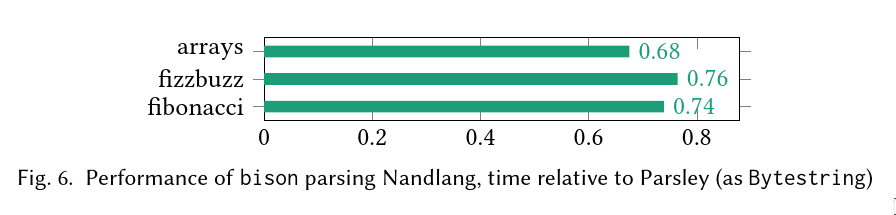
\includegraphics[scale=.6]{pictures/benchmark1Screen.png}
\end{frame}

\begin{frame}[fragile]
\begin{center}
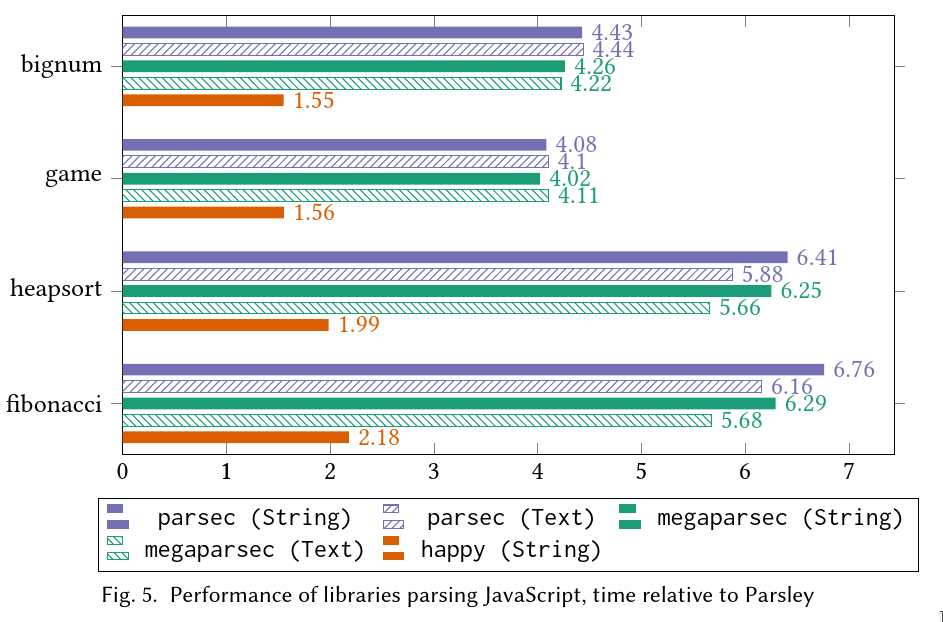
\includegraphics[scale=.5]{pictures/benchmark2Screen.png}
\end{center}
\end{frame}


\section{Заключение}

\begin{frame}{Заключение}
\Large
Достижения:
\begin{itemize}
\item Оптимизированная библиотека персер-комбинаторов с отличной производительностью
\end{itemize}

Задачи на будущее:
\begin{itemize}
\item Обработка ошибок
\item Обход недостатков из-за отсутствия монад:
\begin{itemize}\large
\item Доступ к предыдущим результатам парсинга (например, через "регистры"~\cite{berlin2020})
\end{itemize}
\end{itemize}

\end{frame}

%\begin{frame}{Пути дальнейшего улучшения}
%\begin{itemize}
%\item 1
%\end{itemize}
%\cite{demos}
%\end{frame}

%\begin{frame}
%\begin{center}
%{\Huge Спасибо!}
%\end{center}
%\end{frame}


%\begin{frame}%[t, allowframebreaks]
%\frametitle{Литература}
%\bibliographystyle{amsalpha}
%\bibliography{references}
%\vspace{1cm}
%\end{frame}

\begin{frame}[allowframebreaks]
\frametitle<presentation>{Ссылки}
\begin{thebibliography}{10}

  \bibitem{icfp2020}
    Staged Selective Parser Combinators
    \newblock {\em Jamie Willis \& Nicolas Wu \& Matthew Pickering}
    \newblock \url{https://doi.org/10.1145/3409002}

  \bibitem{berlin2020}
    Garnishing Parsec With Parsley: A Staged Selective Parser Combinator Library
    \newblock {\em Jamie Willis}
    \newblock \url{https://www.youtube.com/watch?v=tJcyY9L2z84}


  \bibitem{selective}
     Selective Applicative Functors
    \newblock {\em Andrey Mokhov \& Georgy Lukyanov \& Simon Marlow \& Jeremie Dimino}
    \newblock \url{https://doi.org/10.1145/3341694}
 
  \bibitem{cuts}
    Библиотека FastParse для Scala
    \newblock \href{https://webcache.googleusercontent.com/search?q=cache:WSoAEDqEOakJ:https://www.lihaoyi.com/fastparse/}{Documentation}
   
  \bibitem{trylookahead}
    Try vs. lookahead
    \newblock \url{https://stackoverflow.com/questions/20020350}
    
%  \bibitem{gerasimov}
%     Курс математической логики и теории вычислимости
%     \newblock {\em Герасимов А.С.}     
%     \newblock \href{https://www.mccme.ru/free-books/gerasimov-3ed-mccme.pdf}{PDF}
%
%  \bibitem{}
%    A Tutorial Introduction to the Lambda Calculus
%    \newblock {\em Ra\'ul Rojas}     
%    \newblock \href{https://www.inf.fu-berlin.de/lehre/WS03/alpi/lambda.pdf}{PDF}
%
%  \bibitem{sicp}
%    Structure and Interpretation of Computer Programs
%    \newblock {\em Abelson, Harold and Sussman, Gerald Jay and {with~Julie~Sussman}}     
%    \newblock \href{https://web.mit.edu/alexmv/6.037/sicp.pdf}{PDF}
%
%  \bibitem{olegSKI}
%    λ to SKI, Semantically (Declarative Pearl)
%    \newblock {\em Oleg Kiselyov}
%    \newblock \href{http://okmij.org/ftp/tagless-final/ski.pdf}{PDF}
    
\end{thebibliography}
 \end{frame}



\end{document}
